\subsection{External interface requirements}
 
	\subsubsection{User Intefaces}
 		SS will feature two different mobille clients: one available to ordinary users and another one dedicated to police officers. Each client will feature a dedicated graphical user interface. \newline
	 In particular the user interface of the police officers client will offer  graphical support for the additional exclusive functions.\newline
		Finally SS will also provide a webpage which will offer access to advanced feature to acknowledge institution.\newline
		The following mockups give an idea of the appearance of the application on release.
	\begin{figure}[h!]
	
	\medskip
	
		\centering
		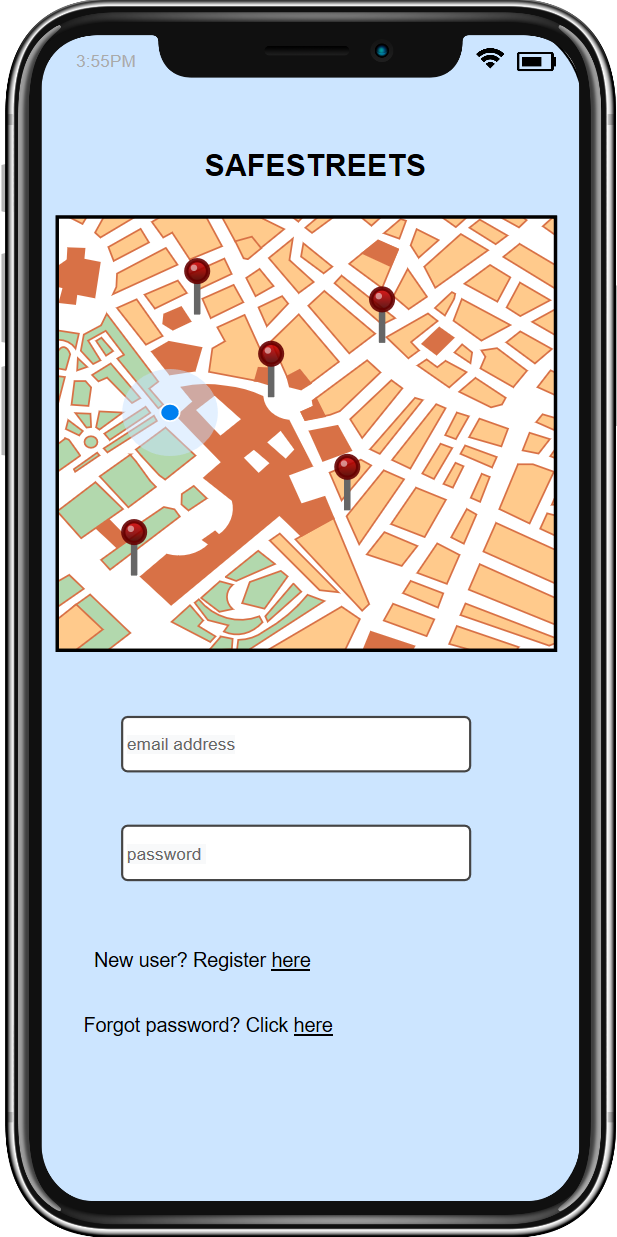
\includegraphics[scale=0.50]{Images/login_mockup}
		\caption{Mockup of the login page}
	\end{figure}
	\newpage
	\begin{figure}[h!]
		\centering
		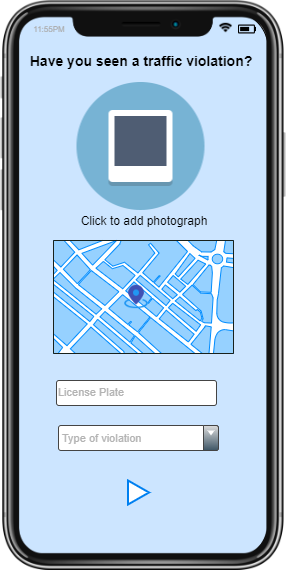
\includegraphics[scale=0.90]{Images/Report_Mockup}
		\caption{Mockup of the form to submit a report}
	\end{figure}
	\newpage
	\begin{figure}[h!]
		\centering
		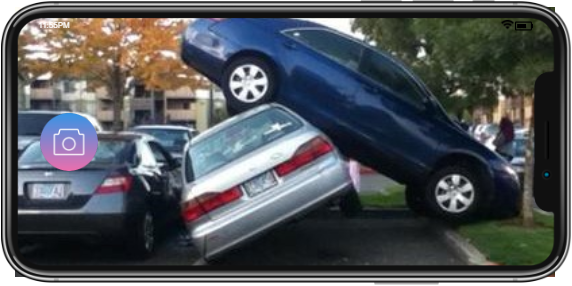
\includegraphics[scale=0.55]{Images/Camera_Mockup}
		\caption{Mockup of the camera interface}
	\end{figure}
	\begin{figure}[h!]
		\centering
		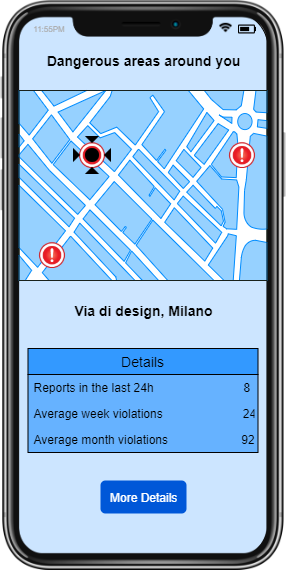
\includegraphics[scale=0.75]{Images/Unsafe_Mockup}
		\caption{Mockup of Unsafe areas page}
	\end{figure}
	\newpage
	\begin{figure}[h!]
		\centering
		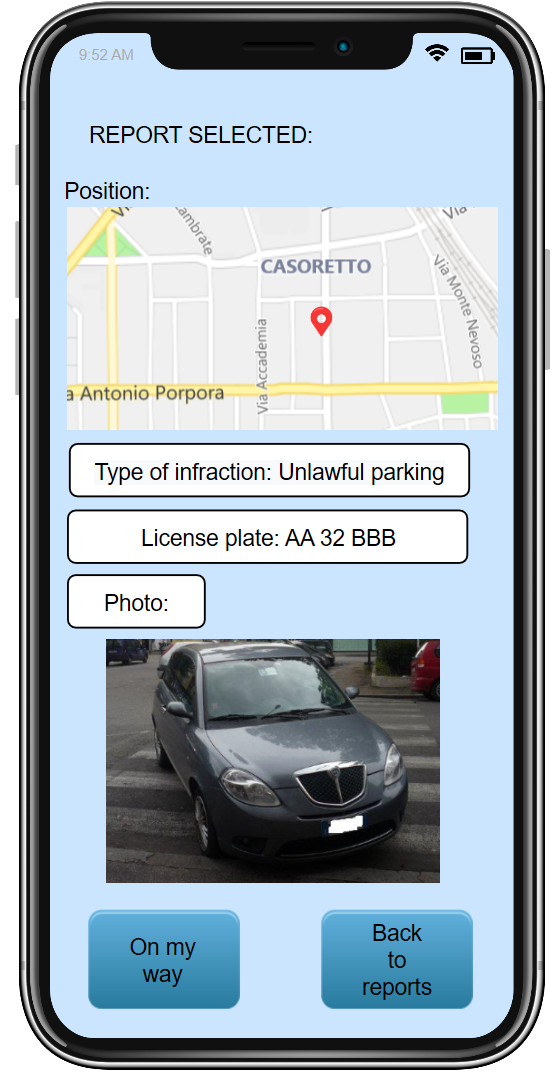
\includegraphics[scale=0.65]{Images/Policeman_client_mockup}
		\caption{Mockup of part of the police client}
	\end{figure}
    \newpage
    \begin{figure}[h!]
    	\centering
    	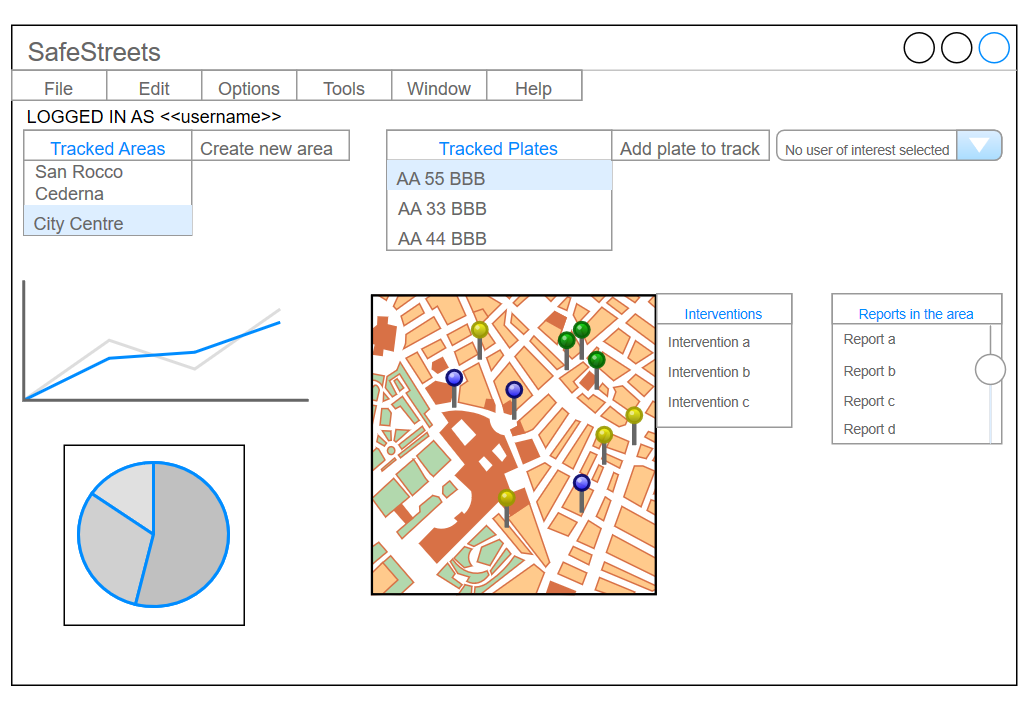
\includegraphics[width=\textwidth]{Images/MunicipalAuthority_client_Mockup}
    	\caption{Mockup of the municipal authority dedicated webpage}
    \end{figure}
    
    \newpage
    
	\subsubsection{Hardware Interface}
	Hardware interfaces are mainly required for the acquisition of the data composing a violation report.
	In particular these represent the necessary interfaces for SS service:
		\begin{itemize}
			\item Smartphone Sensors:\newline
						The access is provided by the APIs and drivers offered by the mobile OS. Those APIs grant the possibility to easly exploit camera and GPS, crucial sensors inside SS user client.
			\item Internet Connection:\newline
						Internet access is vital for the applications since it is entirely based on the comunication between user client and a remote server. So the user client is designed to be installed on a smartphone, assuming that every device will feature an internet module accessible through OS APIs.\newline
						Internet connection is also exploited to retrieve timestamps of each violation and to increase the GPS location accurancy.
	\end{itemize}

	\subsubsection{Software Interfaces}
	Software interfaces required by SS user client are represented by the APIs offered by the mobile OS for the management of the aformentioned hardware modules. In particular, access permission and OS level APIs are required for:
	\begin{itemize} 
		\item Camera
		\item GPS
		\item Storage
		\item Internet Connection (full stack)
	\end{itemize}
	Additionally SS client will exploit the APIs of a third party Street Map Service in order to provide to the users feaure like violations statistic per area, maps of violations and so on.\newline
		Looking at the server endpoint of SS service, the development of an high performance DataBase is reguarded as a main concern for the application scope.\newline
	Finally considering the involvement of third parties for the development of advanced feature of this application, is worth noting that the interfaces with external services will be defined in collaboration with representatives of the third parties involved.
	 
	\subsubsection{Comunication Interfaces}
	 The unique (but fundamental) communication interface required for the scope of this application is the internet connection, as pointed out in the previous sections. The system should provide a device agnostic  connection with adeguated performance.\newline
	In order to provide access to  third parties for stored data (mainly for mining purposes), dedicated APIs will be developed and maintained.
	
	\clearpage
	
\subsection{Functional Requirements}
\bigskip

\begin{enumerate} [label = G\arabic* - ]

\item \textbf{Allow users to signal traffic violations}
	\begin{itemize}
	\item (R1) SS user client must provide a registration interface.
	\item (R2) SS must assign a unique ID to each registered user.
	\item (R3) SS user client must provide a violation report function.
	\item (R4) SS should verify each report is sent from an existent ID.
	\end{itemize}
	\bigskip
	
\item \textbf{Allow users to include pictures in violation reports}
	\begin{itemize}
	\item (R5) Application must have permission and access to the device camera.
	\item (R6) Pictures should be taken through camera inside the application to ensure protection against manipulations.
	\end{itemize}
	\bigskip
	
\item \textbf{The system must be able to retrieve the geographical position of a violation and add it to the report}
	\begin{itemize}
	\item (R7) Application must have permission and ability to access to GPS service offered by the smartphone device.
	\end{itemize}
	\bigskip
	
\item \textbf{The system must recognise (from pictures) license plates}
	\begin{itemize}
	\item (R8) The system should implement an image recognition algorithm.
	\item (R9) The system should ask the user to manually insert the license plate number of the offender car pictured in the provided photo for data integrity purposes.
	\end{itemize}
	\bigskip

\item \textbf{The system must store user made reports}
	\begin{itemize}
	\item (R10) SS must have a consistent database.
	\item (R11) Every report received has to be saved in SS database.
	\item (R12) SS must ensure that data cannot be tampered with.
	\end{itemize}
	\bigskip
	
\item \textbf{Allow users and authorities to mine information collected by the application}
	\begin{itemize}
	\item (R13) SS should provide an authoriteies dedicated client.
	\item (R14) SS authority client should provide a registration function.
	\item (R15) SS should provide the APIs and the tools to allow mining information by 3rd party.
	\item (R16) SS should implement an automated tool for data analysis and display.
	\end{itemize}
	\bigskip
	\end{enumerate}
	
\begin{enumerate} [label = GA 1.\arabic* - ]

\item \textbf{The system must be able to cross the data collected with information about the accidents coming from the municipality} 
	\begin{itemize}
	\item (R17) The involved municipality should provide incidents data of his metropolitan area.
	\item (R18) Data access interfaces should be provided by municipality or defined by SS designers in collaboration with people from the municipality.
	\item (R19) The system should have already collected a suitable amount of data.
	\end{itemize}
	\bigskip
	
\item\textbf{The system must be able to suggest possible interventions to decrease the risk of violations in unsafe areas}
	\begin{itemize}
	\item (R16) SS should implement an automated tool for data analysis and display.
	\end{itemize}
	\bigskip
\end{enumerate}

\begin{enumerate} [label = GA 2.\arabic* - ]
	
\item \textbf{Allow the local police to retrieve data about violation to generate traffic tickets}
	\begin{itemize}
	\item (R20) SS should provide a dedicated client to police officers.
	\end{itemize}
	\bigskip
	
\item \textbf{The system must be able to ensure the veracity of the information sent by the users}
	\begin{itemize}
	\item (R2) SS must assign a unique ID to each registered user.
	\item (R3) SS should verify each report is sent from an existent ID.
	\item (R21) SS should include anti-flooding protection mechanism (e.g. timer for each ID).
	\item (R6) Pictures should be taken through camera inside the application to ensure protection against manipulations.
	\item (R22) Report forward to DB should exploit a secure and encrypted channel.
	\end{itemize}
	\bigskip

\item \textbf{The system must track whether the police has taken care of a certain violation}
	\begin{itemize}
	\item(R23) SS policeman client should offer a function to signal that a traffic ticket (related to a previous) has been generated.
	\item(R24) SS stores in its DB traffic ticket emission alongside the corresponding report.
	\end{itemize}
	\bigskip
	
\item \textbf{Traffic tickets must be issued to the person that owns the vehicle that committed the violation}
	\begin{itemize}
	\item(R25) The system must ensure that the traffic ticket emission signalling (policemen client) is available only for taken care reports.
	\item(R26) SS will ask the officer the license plate number and will accept to signal ticket emission only if the inserted number match the one contained in the report.
	\end{itemize}
	\bigskip
	
\item \textbf{The system must be able to build statistics from the information about issued tickets}
	\begin{itemize}
	\item(R16) SS should implement an automated tool for data analysis and display.
	\end{itemize}
	\bigskip
	
	\end{enumerate}

	\subsubsection{Scenarios}
	\begin{enumerate}
	\item \textbf{Bad Parking}: Bob is a commuter and every morning needs to reach the train station by car: the daily struggle to park his car in the surroundings is even worsened by parking violations. One morning, coming across another car occupying two parking slots, Bob decides to start contributing to SafeStreet service and its violation map: he downloads and installs SS app, accepts to grant Camera and GPS authorizations to it and fills a brief form for the registration. Once logged in, he uses the dedicated report feature. He takes a picture of the violation, inserts manually the license plate number and, after the application completes the verification of the inserted data, he sends the violation report, which also includes the GPS location and the current time.
 	\item \textbf{An anxious mother}: every day Laura lets his 12 years old son walk to school by himself. One day she hears about SS, a new app providing information about traffic violation in her city, and thinks that it can be useful to check if her son daily walking route is reasonably safe or not. Using SS violation map, which provides a street level highlight of violation distribution, she finds out that his son usually walks in potentially unsafe streets, with cars parked on sidewalks forcing pedestrians to walk in the middle of the street, and suggests him a new route based on the map provided by SS.
	\item \textbf{Smart Municipality}: Milan municipality is looking for a large data set regarding traffic monitoring for his metropolitan area. The administration aims to mine useful information from it in order to identify critical areas and plan interventions. They found out SS and its violation DB, so they subscribe to the service as a public institution filling a required form and gain access to the needed data. With high privilege data access granted to public authorities, SS provide them a suitable amount of data for the administration goal.
	\item \textbf{Traffic Monitoring Service}: Gotham City municipality has just introduced a new traffic plan in one of his main districts and wishes to track in an accurate way the evolution of traffic violations. SS should do the trick: Gotham municipality registers to SS service as public authority and now can have privileged access to the data collected by the application. However, Gotham City has no infrastructure dedicated to large data set mining. No worries: the impact of the new traffic plan can be evaluated exploiting built-in SS violation map and traffic tickets emission trends.
	\item \textbf{SafeStreet for Safer Cities}: the city of Monza provide a dedicated service offering data about incidents on its territory. SS has exploited its advanced features to cross its own information about traffic in Monza with the data provided, identifying possible unsafe areas and suggesting possible interventions. The administration of the city knows that managing the traffic plan of a vast city is complex and find that SS automated analysis could really lower effort and costs of the operations. Thus, the municipality decides to register to SS services and to exploit its traffic monitoring and intervention suggestion tool. 
	\item \textbf{Traffic Tickets}: NotSoSafe City is struggling trying to guarantee a decent level of violation control in his vast metropolitan area, considering his personnel available is limited. The municipality come to know that SS provide an efficient violation signalling service and a dedicated police officer client that even tracks ticket emissions. After registration as a public institution, the municipality issue to every policeman the installation of SS client on corporate (or personal) phone. Policemen can now take advantage of the real-time violation notification service of SS app for quick interventions if needed. Moreover, SS violation map offers the municipality a strong tool to simplify territory control: officer patrol activity can be directed to the most unsafe areas reported by the application.
	\item  \textbf{Policeman Intervention}: Anna is a police officer working for Rome municipality. The city administration has recently decide to exploit SS service in order to optimize traffic ticket emission. Anna is patrolling district one and suddenly receive a violation notification from SS client installed on her smartphone. The report is coming from a nearby street so Anna decide to take care of the report, marking that an officer has been dispatched  through the dedicated app function. Once on place, Anna verifies that the violation reported has truly occurred and issues a traffic ticket. She finally marks the report as” taken care” within SS app and gets back to her patrolling activity.
	\end{enumerate}
	
	
	\subsubsection{Use Case Description}
	\medskip
	
	\begin{enumerate}
	\item \textbf{User Registration}
		\begin{table}[h!]
		\centering
		\begin{tabular}{|l|p{12,5cm}|}
		\hline
		Actors            			&       	User\\ \hline
		Goals             			&         G1\\ \hline
		Entry Conditions  	&  		User opens the mobile app for the first time\\ \hline
		Event Flow        		&          
				\begin{enumerate}[label=\alph*)]
					\item The user accepts to grant SS permission to access camera and GPS.
					\item SS user interface shows a menu with Log In and Sign Up options.
					\item The user taps on Sign Up opening the registration form.
					\item The user fills at least the mandatory fields with required personal information.
					\item The user accepts SS privacy policy by ticking a box.
					\item The user confirms the registration by cliking on a link sent to the inserted e-mail account.
				\end{enumerate}\\ \hline
		Output Conditions &    		The user completes the registration and can access SS features.	\\ \hline
		Exceptions        		&       	
				\begin{enumerate}[label=\alph*)]
					\item The user does not accept required permissions. In this case the app will close.
					\item The user is already registered. An error message is displayed asking to reinsert the data is displayed.
					\item Mandatory fields are left empty or filled with invalid entries. An error message is displayed asking to reinsert the data is displayed.
					\item The user does not accept privacy policy. An error message is displayed asking to accept the policy is displayed.
					\item Verification link expires before user confirms registration. In this case the account is deleted from SS system.
				\end{enumerate}\\ \hline
	\end{tabular}
	\end{table}
	
	\clearpage
	
	\item \textbf{Institution Registration}
		\begin{table}[h!]
		\centering
		\begin{tabular}{|l|p{12,5cm}|}
		\hline
		Actors            			&       	Institution/Authority\\ \hline
		Goals             			&         	G6, GA2.1\\ \hline
		Entry Conditions  	&  		No entry condition\\ \hline
		Event Flow        		&          
				\begin{enumerate}[label=\alph*)]
					\item The institution connects to SS website.
					\item In the website institution dedicated area, the authority finds a mandatory registration form. A certificate for institution acknowledgement must be provided as part of the form.
					\item The institution fills all the mandatory fields and accepts privacy policy.
					\end{enumerate}\\ \hline
		Output Conditions &    		Registration successfull: the institution can access advanced SS features.\\ \hline
		Exceptions        		&
				\begin{enumerate}[label=\alph*)]
					\item The institution is already registered.
					\item Mandatory fileds are incomplete.
					\item Certificate is missing.
					\item The institution does not accept Privacy policy.
				\end{enumerate}
				All exceptions raise an error asking to complete the unfulfilled operations. \\ \hline
	\end{tabular}
	\end{table}
	
	\item \textbf{Violation Signaling}
		\begin{table}[h!]
		\centering
		\begin{tabular}{|l|p{12,5cm}|}
		\hline
		Actors            			&       	User\\ \hline
		Goals             			&         G1, G2, G3, G4, G5	\\ \hline
		Entry Conditions  	&  		User is registered, logged in the mobile app and wants to signal a violation\\ \hline
		Event Flow        		&          
				\begin{enumerate}[label=\alph*)]
					\item The user opens SS app and taps on the "Signal a Violation" option.
					\item The user selects one of the possible violations presented in graphic menu.
					\item The app asks the user to attach a photo of the violation, picturing the vehicle involved with license plate visible, and to manually insert license plate number of the vehicle.
					\item The user takes a photo of the violation within SS app and insert license plate number of the vehicle.
					\item The app localy verifies if the license plate pictured and the manually inserted one match and readies the violation report. 
					\item The app shows a menu displaying a " Send Report" and a "Cancell" options.
					\item The user tap on "Send Report" in order to send the violation report to SS systems.
					\end{enumerate}\\ \hline
		Output Conditions &    		The report is sent to SS server and it is stored in a suitable database.\\ \hline
		Exceptions        		&       	
				\begin{enumerate}[label=\alph*)]
					\item License plate number recognized by the app and the one manually inserted do not match. In this case, an error message is raised and SS asks the user to retake the photo.
				\end{enumerate}\\ \hline
	\end{tabular}
	\end{table}
	
	\item \textbf{Providing Useful Information to Users}
		\begin{table}[h!]
		\centering
		\begin{tabular}{|l|p{12,5cm}|}
		\hline
		Actors            			&       	User\\ \hline
		Goals             			&         G6, GA2.5\\ \hline
		Entry Conditions  	&  		User is registered, logged in the mobile app and wants to consult violation information\\ \hline
		Event Flow        		&          
				\begin{enumerate}[label=\alph*)]
					\item The user opens SS app and taps on the "Statistics" option.
					\item The user selects the prefered function in the menu displayed (e.g. violations maps, traffic tickets statistics). \newline
								Note: functions availability may vary depending on the service offered by the city municipality.
				\end{enumerate}\\ \hline
		Output Conditions &    		The user acess to the requested service.\\ \hline		
				
		Exceptions        		&       	
				\begin{enumerate}[label=\alph*)]
					\item The user requests a service not available in his city. An error message explaining the reasons of the function absence is displayed.
				\end{enumerate}\\ \hline
	\end{tabular}
	\end{table}
	
	\item \textbf{Providing Data to Mine to Istitutions}
		\begin{table}[h!]
		\centering
		\begin{tabular}{|l|p{12,5cm}|}
		\hline
		Actors            			&       	Institution/authority\\ \hline
		Goals             			&         	G6\\ \hline
		Entry Conditions  	&  		Institution is registered to SS service and desires to access to data it collects\\ \hline
		Event Flow        		&          
				\begin{enumerate}[label=\alph*)]
					\item The institution specifies a proper query for the data required.
					\item The system verifies if the query author is an registered acknowledge.
					\end{enumerate}\\ \hline
		Output Conditions &    		Requested data is provided to the institution. \\ \hline
		Exceptions        		&
		       	\begin{enumerate}[label=\alph*)]
		       		\item The query is not well formatted. An error is reported and the transaction is aborted.
		       		\item The query author is not recognized. An error is reported and the request is not fullfilled. 
		       	\end{enumerate}\\ \hline
	\end{tabular}
	\end{table}
	
		\clearpage
	
	\item \textbf{Providing Institution Intervention Suggestions}
		\begin{table}[h!]
		\centering
		\begin{tabular}{|l|p{12,5cm}|}
		\hline
		Actors            			&       	Institution/Authority\\ \hline
		Goals             			&         	GA1.2\\ \hline
		Entry Conditions  	&  		Institution is registetred to SS service and desires to access to "Suggested Intervention" advanced feature\\ \hline
		Event Flow        		&          
				\begin{enumerate}[label=\alph*)]
					\item The institution logs in the SS website
					\item The institution navigates to the "Suggested Intervention" sections
					\item In the interface displayed the institution searches the areas of interest for possible intervention suggestions
					\end{enumerate}\\ \hline
		Output Conditions &    		The institution can access to intervention suggestions for the selected area\\ \hline
		Exceptions        		&       	
				\begin{enumerate}[label=\alph*)]
					\item The institution fails to login in the website page. An error message asking to reinsert credential is displayed.
					\item In the selected area there are no suggested intervention. An error message explaining the absense of possible intervention is reported.
				\end{enumerate}\\ \hline
	\end{tabular}
	\end{table}
	
	\item \textbf{Police Officer Takes Care of a Report}
		\begin{table}[h!]
		\centering
		\begin{tabular}{|l|p{12,5cm}|}
		\hline
		Actors            			&       	Police Officer\\ \hline
		Goals             			&         	GA2.1, GA2.3\\ \hline
		Entry Conditions  	&  		The police officer receives a notification on her/his SS mobile client and decides to take action\newline
													\centerline{OR}\newline
													The police officers finds in the SS client dedicated section an available violation report and decides to take care of it \\ \hline
		Event Flow        		&          
				\begin{enumerate}[label=\alph*)]
					\item The police officer taps on the notification (selects a violation report).
					\item The app shows the report and two option: "On my Way", to take over the violaton report; "Back to Reports", to come back to violations map.
					\item The police officer selects "On my way" option.
					\item The police officer reaches the location indicated in the violation reports.
					\item The police officer verifies if the signaled violation has truly occurred and in this case emits a traffic ticket.
					\item The police officer concludes intervention specifying its outcome in SS app, through the options displayed: "Ticket emitted" or "Violation not verified". 
					\end{enumerate}\\ \hline
		Output Conditions &    		In case of verified violation, a ticket emission is stored with the corresponding violation. Otherwise, the violation record is removed from SS systems.\\ \hline
		Exceptions        		&       	
				\begin{enumerate}[label=\alph*)]
					\item A colleague takes over the violation before the policeman selects "On my way" option. An error message stating that the violation is already under analisys is displayed.
				\end{enumerate}\\ \hline
	\end{tabular}
	\end{table}
	
	
	\end{enumerate}
	
	\subsubsection{Use Case Diagram}
	\begin{figure}[h!]
		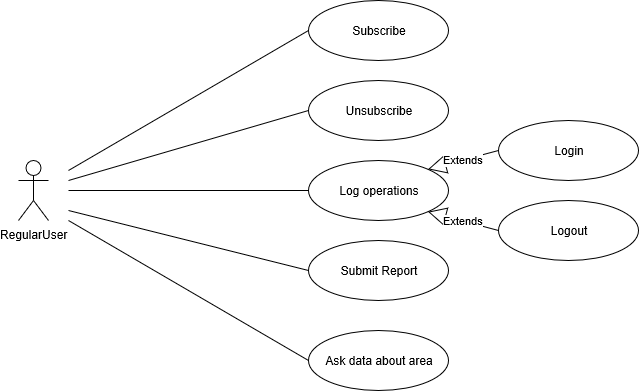
\includegraphics[scale=0.65]{Images/UseCaseDiagram-RegularUser}
		\caption{Regular user}
	\end{figure}
	\begin{figure}[h!]
		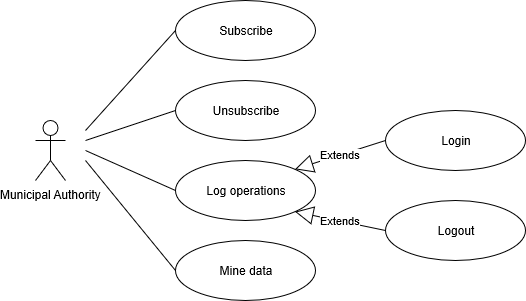
\includegraphics[scale=0.65]{Images/UseCaseDiagram-MunicipalAuthority}
		\caption{Municipal Authority}
	\end{figure}
\newpage
	\begin{figure}[h!]
		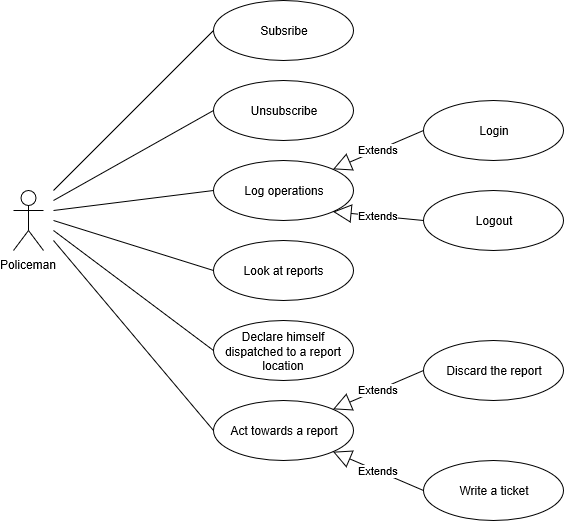
\includegraphics[scale=0.75]{Images/UseCaseDiagram-Policeman}
		\caption{Policeman}
	\end{figure}
\newpage
	
	\subsubsection{Sequence Diagrams}
	\begin{figure}[h!]
		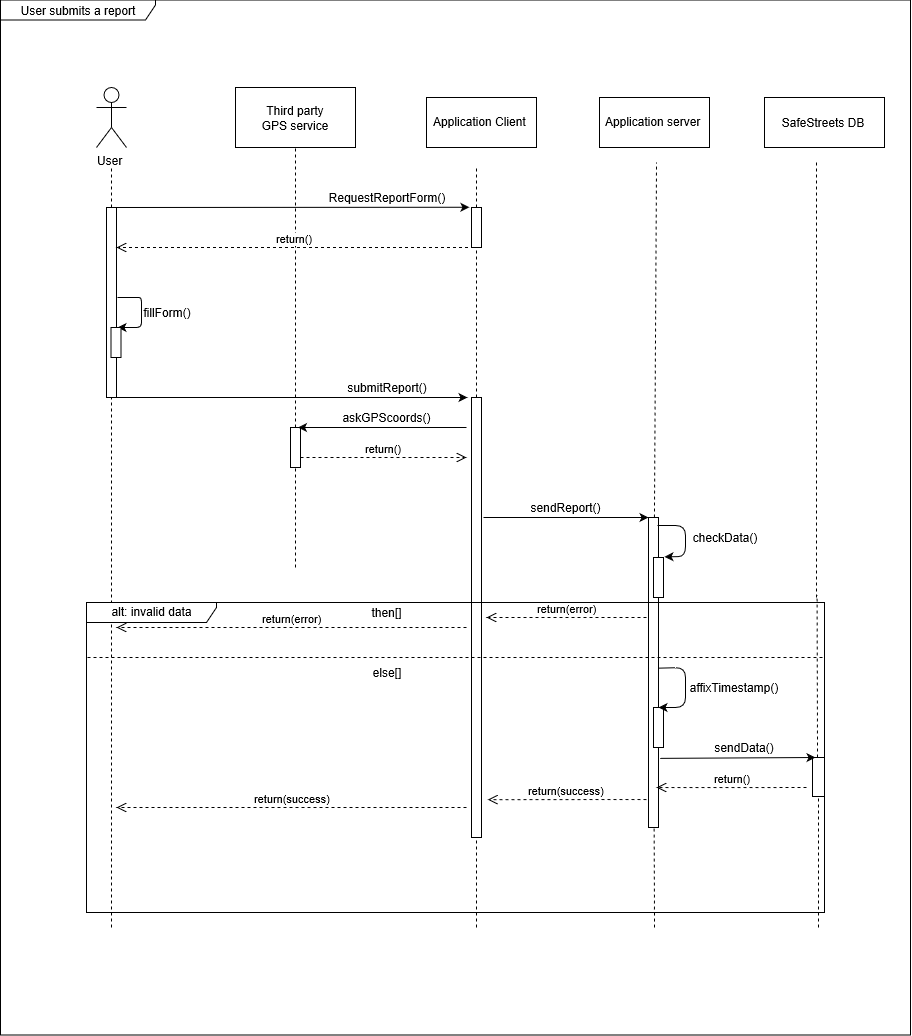
\includegraphics[width=\textwidth]{Images/ReportSubmitSequenceDiagram-0-2}
		\caption{Report submit}
	\end{figure}
	\newpage
	\begin{figure}[h!]
		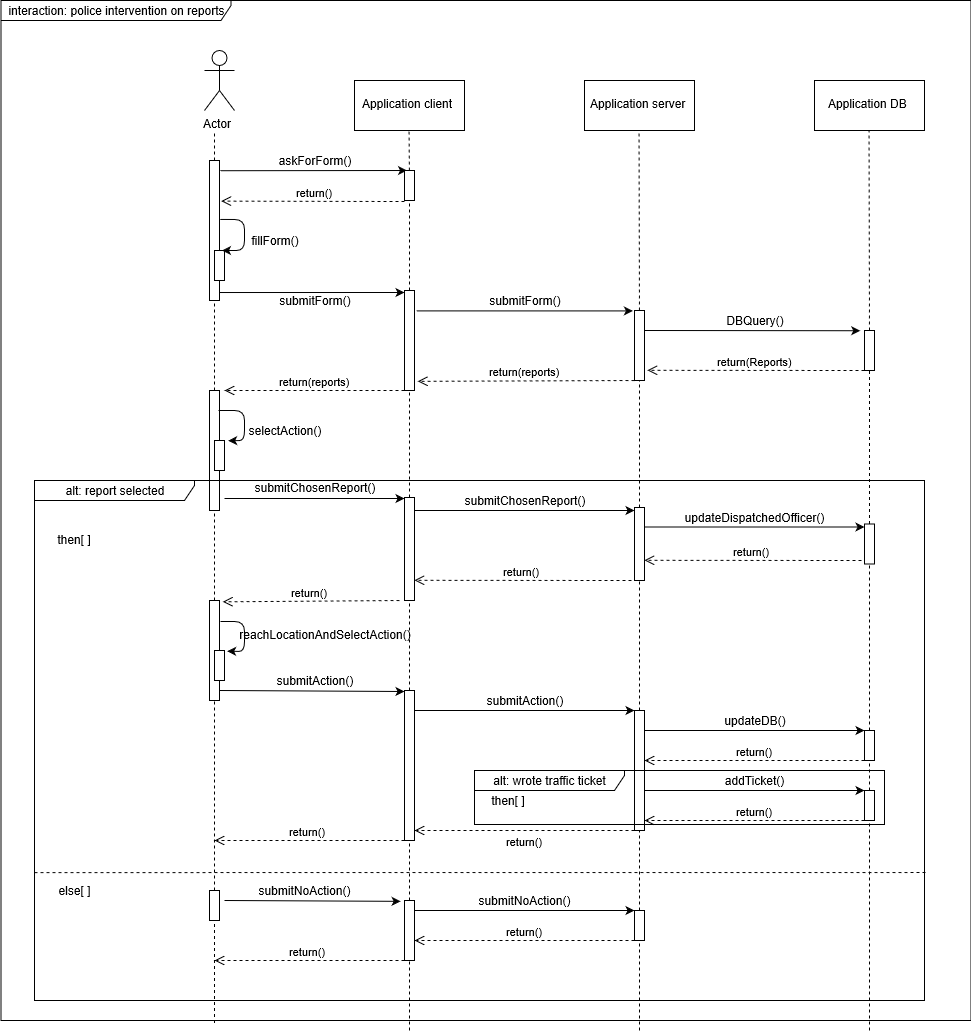
\includegraphics[width=\textwidth]{Images/PoliceIntervention}
		\caption{Police intervention}
	\end{figure}
	\newpage
	\begin{figure}[h!]
		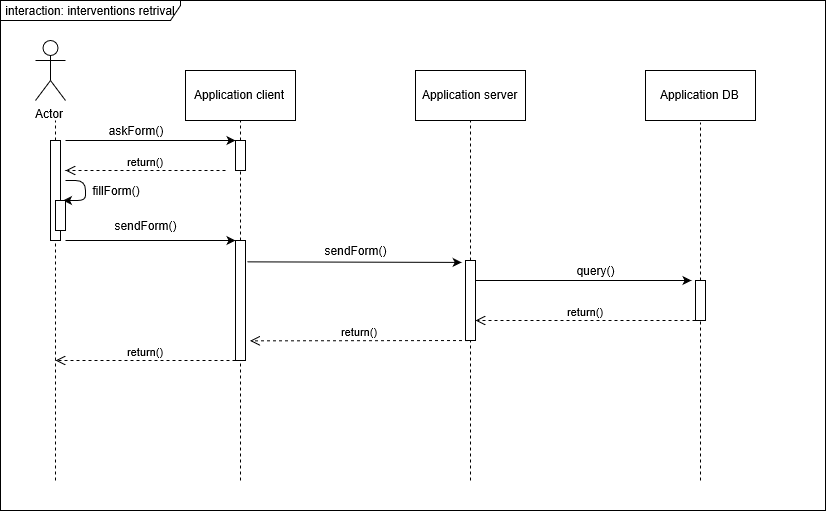
\includegraphics[width=\textwidth]{Images/InterventionRetrivalSequenceDiagram}
		\caption{Intervertion retrival}
	\end{figure}
\newpage
	
	\subsubsection{Mapping on Requirements}
	Here we present the traceability matrix, showing relations among goals, requirements and use case of the application.\newline
	%Note that security requirements are not linked to specific use case since they are related to improper uses of the application
	\medskip
	
	\begin{table}[h!]
	\centering
	\begin{tabular}{|l|l|l|}
	\hline
	\textbf{Goals}					& \textbf{Requirements}	& \textbf{Use Cases}\\ \hline
 	\multirow{4}{*}{G1}		&   	R1 								&  1\\\cline{2-3}
 											& 		R2								&	 1\\\cline{2-3}
 											&   	R3 								&  3\\\cline{2-3}
 											&   	R4 								&  3\\\cline{2-3} \hline
 											
 	\multirow{2}{*}{G2}		&   	R5 								&  3\\\cline{2-3}
 											&   	R6 								&  3\\\cline{2-3} \hline
 											
 	\multirow{1}{*}{G3}		&   	R7 								&  3\\\cline{2-3}\hline
 	
 	\multirow{2}{*}{G4}		&   	R8 								&  3\\\cline{2-3}
 											&   	R9 								&  3\\\cline{2-3} \hline
 											
 	\multirow{3}{*}{G5}		&   	R10 								&  3\\\cline{2-3}
 											&   	R11 								&  3\\\cline{2-3}
 											&   	R12 								&  3\\\cline{2-3}\hline
 											
 	\multirow{4}{*}{G6}		&   	R13 								&  2\\\cline{2-3}
 											&   	R14 								&  2\\\cline{2-3}
 											&   	R15 								&  5\\\cline{2-3}
 											&   	R16 								&  5\\\cline{2-3}\hline
 											
	\multirow{3}{*}{GA1.1}	&   	R17 								&  6\\\cline{2-3}
											&   	R18 								&  6\\\cline{2-3}
											&   	R19 								&  6\\\cline{2-3} \hline
											
 	\multirow{1}{*}{GA1.2}	&   	R16 								&  6\\\cline{2-3} \hline
 	
 	\multirow{1}{*}{GA2.1}	&   	R20 								&  7\\\cline{2-3} \hline
 	
 	\multirow{5}{*}{GA2.2}	&   	R2 								&  \\\cline{2-3} 
 											& 		R3 								&  \\\cline{2-3} 
 											&		R21 								&  \\\cline{2-3} 
 											&		R6 								&  \\\cline{2-3}
 											&		R22 								&  \\\cline{2-3}\hline
 									
 	\multirow{2}{*}{GA2.3}	&  	R23 								&  7\\\cline{2-3}
 											&  	R24 								&  7\\\cline{2-3} \hline
 											
 	\multirow{2}{*}{GA2.4}	&  	R25 								&  7\\\cline{2-3}
 											&  	R26 								&  7\\\cline{2-3} \hline
 											
 	\multirow{1}{*}{GA2.5}	&  	R21 								&  5\\\cline{2-3}\hline
	\end{tabular}
	\end{table}
	
	\newpage
	
\subsection{Performance Requirements}

	\subsubsection{Response time}
	
Server side SS is a data intensive application. Big volumes of data  will be written and read at the same time. Given the nature of the application itself, fast responses are essential in order to make the policemen do their job properly. On the data analytics side, instead, the responses can be slower.\\

\textbf{List of the response times:}
\begin{itemize}
\item report forwarded to application DB: 500 ms, medium priority
\item response to policeman query on DB: 500ms, medium priority
\item responses to policemen actions insertion in DB: 200 ms, high priority
\item responses to regular users queries on data: 500 ms, low priority
\item responses to municipal authorities data-mining actions: 1 min, low priority
\end{itemize}
\subsubsection{Workload management}
SS will need to be able to sustain a heavy workload of database transaction: there will be a lot of simultaneous read and write operations. The workload required will differ depending on the differnt types of users.
\begin{itemize}
	\item \textbf{Regular Users:} the number of data streams will vary greatly depending on the number of users and the size of the city immplementing SS. As a safety measure, supposing to implement SS in a city roughly se same size as Milano, the number of expected data streams could exceed 100'000 daily, considering both reads and writes
	\item \textbf{Police Officers: } given the relative small number of municipal and police employees, a good extimate in a city the size of Milano could be around 2000 data streams daily on average, insignificant when compared to the other users' streams  
\end{itemize}
In conclusion, it's evident that SS must be able to scale seamlessly and in an automated fashion, without human intervention


\subsection{Design Constraints}
	\subsubsection{Standard Compliance}
	SS mobile client should respond to the following requirements:
	\begin{itemize}
		\item[--] The application saves the current state when it is put in backgound or when the smartphone enter standby mode; it restores all the saved states when is called to the foreground.
		\item[--] The application works flawlessly in an SD card, provided space is available.
		\item[--] The application can be used either on landscape or portrait orientations.
	\end{itemize}
	The system to be delivered must comply with EU's GDPR (General Data Protection Regulation) and will follow any of its variations in the time to come.
	\subsubsection{Hardware Limitations}
	SS will have really different hardware limitations client side and server side:
	\begin{itemize}
		\item \textbf{Client side}:
		\begin{itemize}
		 \item[--] Mobile Client: the only limitation is a working smartphone featuring a working camera, a GPS location module and an internet connection.
		 \item[--] WebPage: working device with internet connection.
		 \end{itemize}
		\item \textbf{Server side} - SS will need to save huge amounts of data, thus needing huge amounts of reliable storage
	\end{itemize}
	 
\subsection{Software System Attributes}
	\subsubsection{Reliability}
	Given the data-mining orientation of the application, a huge amount of data must be gathered in order to ensure that the statistic analysis on the aformentioned data is actually meaningful. Therefore, the system must be reliable in delivering un-compromised data to the database and reliably store them.\\
	It is also necessary for the system to accurately update dispatched officers and what reports have been taken care of, in order to avoid an erroneous usage of municipal police manpower and time, whose are usually pretty low to begin with.
	\subsubsection{Avaibility}
	Once again, in order to gather enough information to produce meaningful statistical analysis, the system must be able to gather as much data as possible. In order for this to happen the system must have a high availability, in the order of .9999
	\subsubsection{Security}
	Given that SS deals with a high volume of sensible data, such as pinpointing a user to a certain place at a certain time or having a list of various tickets emitted by the police, it is of the utmost importance for it to have a robust security apparatus. As a starter, all comunications between client and server must be encrypted (an asymmetric encryption mechanism with hash check should be enough); the same goes for the stored data. Other measures to be taken in order to avoid data leaks are the usual ones: don't use obvious names for tables and columns, filter all the user input, use adeguate csp to avoid code injections, use anti CSRF tokens and so on.\\
	Please note that a leak could have disastrous consequences both on reputation and economic level, therefore security's importance cannot be understated and has to be considered one of the top priorities. 
	\subsubsection{Mantainability}
	The greatest challenge in the maintanability field lays in the correct application of the "divide et impera" principle: if the application's modules have been defined and developed correctly then mantaining each module will be feasible with little cost in time and effort.
	\subsubsection{Portability}
	Portability is a relatively easy problem to solve. As a matter of fact, given that the users will access SS via a smartphone client, it will be enough to develop clients for Andorid and IOS and keep it updated to keep up with new os version releases. 
